\section{Statics vs Dynamics of a Spring-Damper Mass System}

he system consists of a point mass $m$ located at position $\vec{r}_C = [x, y]^\top$.
Gravity $g$ acts in the downward direction, denoted as $-g\hat{j}$.

Two anchor points, $A$ and $B$, are fixed at $\vec{r}_A$ and $\vec{r}_B$, respectively.
The mass is connected to each anchor by a spring and a dashpot arranged in parallel:
\begin{itemize}
    \item \textbf{Anchor A:} Connected via a spring with constant $k_A$ and rest length $L_A$, and a parallel dashpot with damping coefficient $c_A$.
    \item \textbf{Anchor B:} Connected via a spring with constant $k_B$ and rest length $L_B$, and a parallel dashpot with damping coefficient $c_B$.
\end{itemize}

Additionally, the mass is subject to an atmospheric drag force proportional to its speed through the air, characterized by the damping coefficient $c_d$.

The dynamic state of the system is described by the vector $z = [x, y, v_x, v_y]^\top$, while the static equilibrium state is defined by $z = [x, y, 0, 0]^\top$.

The system may be described using Newton's Second Law of Motion with the vector equation

\begin{equation}
    m \frac{d^2\vec{r}_c}{dt^2} = -mg\hat{j} + \left[ k_A\delta_A + c_A \left( \frac{d\vec{l}_A}{dt} \cdot \hat{a} \right) \right] \hat{a} + \left[ k_B \delta_B + c_B \left( \frac{d\vec{l}_B}{dt} \cdot \hat{b} \right) \right] \hat{b} - c_d \frac{d\vec{r}_c}{dt}
    \label{Eq:System9}
\end{equation}

where

\begin{eqnarray}
    \vec{r}_c & = & \vec{r}_{A/B} + \big( \vec{L}_{A/B} + \vec\delta_{A/B} \big) \\
    \vec{l}_{A/B} & = & \vec{L}_{A/B} + \vec\delta_{A/B} \nonumber \\
    \vec{a} & = & \vec{r}_c - \vec{r}_A \nonumber \\
    \vec{b} & = & \vec{r}_c - \vec{r}_B \nonumber
    \label{Eq:System9_helper}
\end{eqnarray}

and any vector $\vec{v} = ||v|| \; \hat{v}$.

In the static limit, this equation simplifies to

\begin{equation}
    mg \; \hat{j} = k_A\delta_A \; \hat{a} + k_B\delta_B \; \hat{b}.
\end{equation}

\begin{minted}{julia}
function get_dparameters(sys::fparameters, r_c::Vector{Float64})
    a_vec = sys.rₐ - r_c
    b_vec = sys.rᵦ - r_c

    # Current scalar lengths
    lₐ_val = norm(a_vec)
    lᵦ_val = norm(b_vec)

    return dparameters(lₐ_val, lᵦ_val, a_vec, b_vec)
end

# ---- Define System Evolution ---- #

function spring_damper_mass_system!(du, u, p, t)
    # Unpack state
    r_c = u[1:2]
    v_c = u[3:4]

    # Unpack Parameters
    m = p.m
    r_A, r_B = p.rₐ, p.rᵦ

    k_A, k_B = p.kₐ, p.kᵦ
    L_A, L_B = p.Lₐ, p.Lᵦ

    c_A, c_B, c_d = p.cₐ, p.cᵦ, p.c_d

    # -- Geometry -- #
    vec_to_A = r_A - r_c
    vec_to_B = r_B - r_c

    dist_A = norm(vec_to_A)
    dist_B = norm(vec_to_B)

    # Unit Vectors
    hat_A = vec_to_A / dist_A
    hat_B = vec_to_B / dist_B

    # -- Force Calculations -- #

    # - Springs - #
    delta_A = dist_A - L_A
    delta_B = dist_B - L_B

    F_spring_A = k_A * delta_A * hat_A
    F_spring_B = k_B * delta_B * hat_B

    # - Dampers - #
    vel_proj_A = dot(v_c, -hat_A)
    vel_proj_B = dot(v_c, -hat_B)

    F_damp_A = -c_A * dot(v_c, hat_A) * hat_A
    F_damp_B = -c_B * dot(v_c, hat_B) * hat_B

    # - Drag - #
    F_drag = -c_d * v_c

    # - Gravity - #
    F_gravity = [0.0, -m * g]

    # -- Newton's Second Law -- #

    F_total = F_spring_A + F_spring_B + F_damp_A + F_damp_B + F_drag + F_gravity
    accel = F_total / m

    # -- Update State -- #
    du[1:2] = v_c    # dr/dt = v
    du[3:4] = accel  # dv/dt = F/m

end

# Initial Conditions
u0 = [5.0, 0.0, 0.0, 2.0]

# Time Span
tspan = (0.0, 50.0)

prob = ODEProblem(spring_damper_mass_system!, u0, tspan, params)
sol = solve(prob, Tsit5(), saveat=0.1)

phase_space = plot(sol, idxs=(1,2),
     title="Mass Trajectory",
     xlabel="x position (m)",
     ylabel="y position (m)",
     label="Path", lw=2, aspect_ratio=:equal)

# ---- Solving for a Static System ---- #

function static_forces!(F, r_c, sys::fparameters)
    a_vec = sys.rₐ - r_c
    b_vec = sys.rᵦ - r_c

    lₐ = norm(a_vec)
    lᵦ = norm(b_vec)

    hat_a = a_vec / lₐ
    hat_b = b_vec / lᵦ

    delta_a = lₐ - sys.Lₐ
    delta_b = lᵦ - sys.Lᵦ

    gravity = [0.0, -sys.m * g]
    force_a = sys.kₐ * delta_a * hat_a
    force_b = sys.kᵦ * delta_b * hat_b

    # Update the F array in-place
    F[1] = gravity[1] + force_a[1] + force_b[1]
    F[2] = gravity[2] + force_a[2] + force_b[2]
end

# ---- Generate Steady State Solution Clusters ---- #

num_samples = 2000
solutions_x = Float64[]
solutions_y = Float64[]

# Wrap the function so NLsolve only sees F and x
target_func!(F, x) = static_forces!(F, x, params)

for i in 1:num_samples
    x0 = -5.0 + 20.0 * rand()
    y0 = -10.0 + 25.0 * rand()
    initial_guess = [x0, y0]


    res = nlsolve(target_func!, initial_guess, autodiff=:forward, ftol=1.5)

    # If successful, save the raw, unrounded coordinates
    if converged(res)
        push!(solutions_x, res.zero[1])
        push!(solutions_y, res.zero[2])
    end
end


# ---- Custom Steady State Clustering Algorithm ---- #
# Combine points for easier handling
points = tuple.(solutions_x, solutions_y)

# Round off to integers and find unique classes
rounded_points = tuple.(round.(Int, solutions_x), round.(Int, solutions_y))
unique_classes = unique(rounded_points)

println("Identified $(length(unique_classes)) integer class seeds.")

# Create a dictionary to hold the assigned points for each class
clusters = Dict(c => Tuple{Float64, Float64}[] for c in unique_classes)

# Assign each original point to the nearest integer class using Euclidean distance
for p in points
    best_class = unique_classes[1]
    min_dist = Inf

    for c in unique_classes
        # Euclidean distance formula
        dist = sqrt((p[1] - c[1])^2 + (p[2] - c[2])^2)
        if dist < min_dist
            min_dist = dist
            best_class = c
        end
    end
    push!(clusters[best_class], p)
end

# Centroids of each newly formed class
centroids_x = Float64[]
centroids_y = Float64[]

for (class_seed, cluster_points) in clusters
    if !isempty(cluster_points)
        # Calculate mean of X and Y
        cx = sum(p[1] for p in cluster_points) / length(cluster_points)
        cy = sum(p[2] for p in cluster_points) / length(cluster_points)

        push!(centroids_x, cx)
        push!(centroids_y, cy)

        println("Region Centroid: (X: $(round(cx, digits=4)), Y: $(round(cy, digits=4)))")
    end
end
\end{minted}

Solving for this system using a 5th order solver (TSit), one may observe obvious signs of a chaotic system

\begin{itemize}
    \item Sensitivity to initial conditions.
    \item Strange attractors in the phase space (clearly visible)
    \item Open loops (aperiodicity) in the phase space.
\end{itemize}

\begin{figure}[!h]
    \centering
    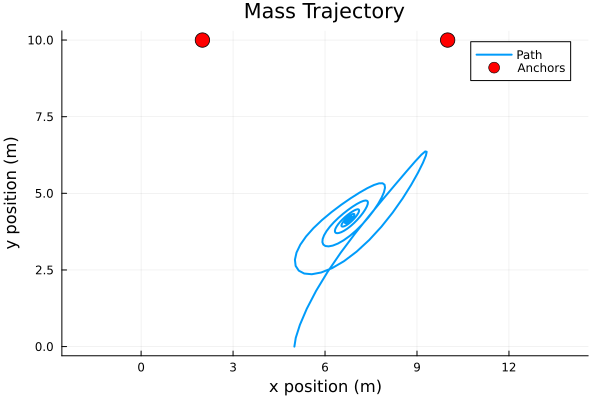
\includegraphics[width=0.8\linewidth]{Problems/Problem13/figures/chaos1.png}
    \caption{TSit Numerical Solution -- Phase Space}
    \label{fig:placeholder}
\end{figure}

One may use Julia's NLsolve (similar to MatLab's fsolve) to identify the system's static solutions. The system is reduced to its static limit and fed into NLsolve, which identified 1737 (unique and non-unique) solutions in 2000 runs. \\
\\

\begin{figure}[!h]
    \centering
    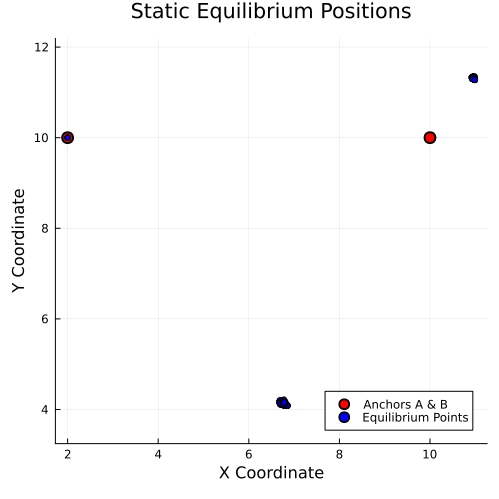
\includegraphics[width=0.4\linewidth]{Problems/Problem13/figures/static_solutions.png}
    \caption{NLsolve Solutions}
    \label{fig:placeholder}
\end{figure}

One can clearly visualize that the solutions are far apart. Given the nature of the clusters, one may forgo using standard clustering algorithms in machine learning (such as KMeans or GMM) in place of much simpler algorithms. Here the following algorithm is used to define clusters.

\begin{enumerate}
    \item All solutions are reduced to their greatest integer forms. This can be done this the the error by NLsolve is smaller than $\mathcal{O}(1)$.
    \item Unique (integral) solutions are identified. Each unique solution is assigned an unlabeled class (or cluster) as a \textit{center point}.
    \item All the (unrounded) solutions from NLsolve are assigned a cluster based on the least Euclidean distance from the respective \textit{center point}.
    \item The centroid of all the points in each cluster is presented a point of equillibrium.
\end{enumerate}

\begin{figure}[h!]
    \centering
    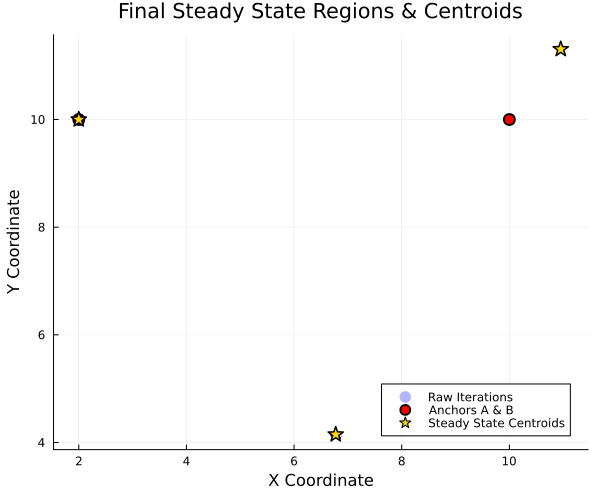
\includegraphics[width=0.4\linewidth]{Problems/Problem13/figures/rounded_static_solutions.png}
    \caption{Clustered NLsolve Solutions for System Statics}
    \label{fig:placeholder}
\end{figure}

\begin{table}[htbp]
    \centering
    \caption{Final Steady State Regions (Centroids)}
    \label{tab:steady_state_centroids}
    \begin{tabular}{ccc}
        \hline
        \textbf{Region} & \textbf{X Coordinate (m)} & \textbf{Y Coordinate (m)} \\
        \hline
        1 & 6.7738 & 4.1472 \\
        2 & 2.0000 & 10.0000 \\
        3 & 10.9523 & 11.3063 \\
        \hline
    \end{tabular}
\end{table}

\subsection{Evaluating Stability : Numerical Simulations}

To evaluate the stability of the discovered fixed points, one may simulate the system with initial positions set to the fixed points and an arbitrarily small velocities to simulate a perturbation. Observing the behaviour of the system (converging back to the fixed point/ diverging from the fixed point) allows one to assess the stability.

In the system simulate here, three distinct fixed points were discovered. The system was simulated (as done above) using TSit5 from the fixed points with varying perturbations. It is discovered that two of the three fixed points are unstable. Following their respective perturbations, all three masses converge at the singular stable fixed point of the system.

\begin{figure}
    \centering
     % --- Row 1 ---
     \begin{subfigure}[b]{0.45\textwidth}
         \centering
         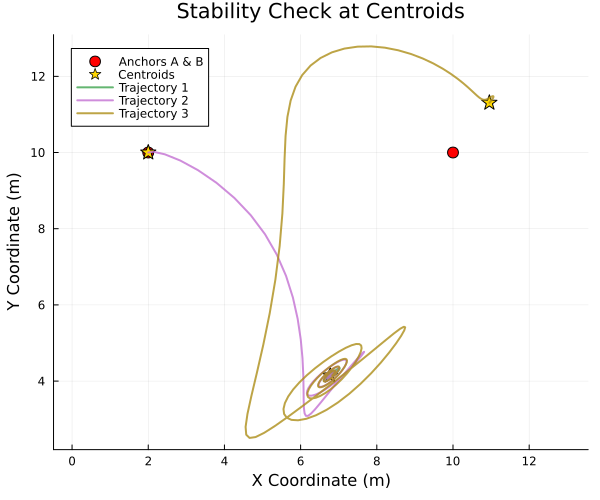
\includegraphics[width=\textwidth]{Problems/Problem13/figures/stability.png}
         \caption{Perturbation of $\vec{v}_0 = (0.5 \;\hat{i}+ 0.5 \;{\hat{j})}\; \text{m/s}$}
         \label{fig:k0}
     \end{subfigure}
     \hfill
     \begin{subfigure}[b]{0.45\textwidth}
         \centering
         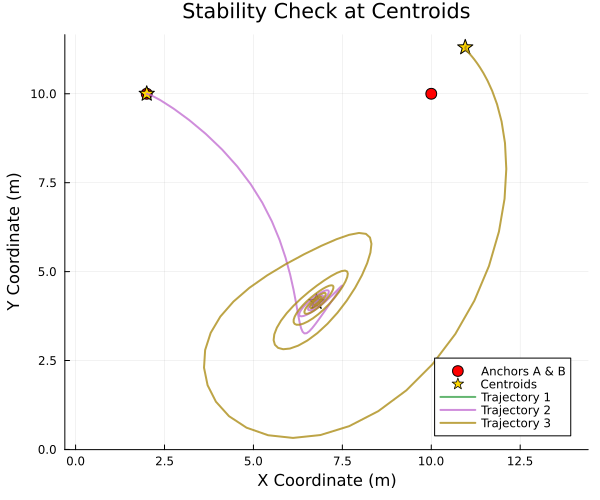
\includegraphics[width=\textwidth]{Problems/Problem13/figures/stability2.png}
         \caption{Perturbation of $\vec{v}_0 = (0.1 \;\hat{i}+ 0.1 \;{\hat{j})}\; \text{m/s}$}
         \label{fig:rigid}
     \end{subfigure}

    \caption{Stability of Discovered Fixed Points}
\end{figure}

\subsection{Evaluating Stability : Jacobians}
Write the equations of motion as $\dot{z}=f(z)$, with $z=[x,y,v_x,v_y]^\top$. A fixed point $z^*=[x^*,y^*,0,0]^\top$ satisfies $f(z^*)=0$. To assess its stability, we ask whether a small disturbance in position or velocity grows or decays with time.

The Jacobian records how each component of $f$ changes when a state variable changes. At the fixed point, its entries are
\begin{equation}
    J_{ij}=\left.\frac{\partial f_i}{\partial z_j}\right|_{z=z^*}.
\end{equation}
For a small disturbance $\eta=z-z^*$, a first-order approximation gives
\begin{equation}
    \dot{\eta}=f(z^*+\eta)\approx f(z^*)+J\eta=J\eta.
\end{equation}
Thus, close to the fixed point, we can study a linear system instead of the full nonlinear equations. Here, $J$ is a $4\times4$ matrix obtained from the full equations of motion, including the damping terms.

\begin{minted}{julia}
function rhs(u)
    du = Vector{eltype(u)}(undef, 4)
    spring_damper_mass_system!(du, u, params, 0.0)
    return du
end

for (i, fp) in enumerate(fixed_points)
    # Compute 4x4 Jacobian Matrix at u* via Forward-Mode AD
    J = ForwardDiff.jacobian(rhs, fp)
    
    # Calculate Eigenvalues
    λ = eigvals(J)
    
    # Stability criterion: all Re(λ) < 0
    is_stable = all(real.(λ) .< 0.0)
    classification = is_stable ? "Asymptotically Stable (Sink)" : "Unstable (Saddle/Source)"
    
    for (j, val) in enumerate(λ)
        re, im = round(real(val), digits=4), round(imag(val), digits=4)
        sign_str = im >= 0 ? "+" : "-"
        println("    λ_$(j) = $re $sign_str $(abs(im))i")
    end
end
\end{minted}

For an eigenvector $q$ of $J$, the associated disturbance in this linear approximation has the form
\begin{equation}
    Jq=\lambda q, \qquad \eta(t)=a e^{\lambda t}q,
\end{equation}
where $a$ sets the initial disturbance size. The real part of $\lambda$ determines growth or decay, while a nonzero imaginary part indicates oscillation. For a smooth system, this gives the following local stability criteria:
\begin{itemize}
    \item If all eigenvalues have negative real parts, small disturbances decay and the fixed point is locally asymptotically stable.
    \item If any eigenvalue has a positive real part, some disturbances grow and the fixed point is unstable.
    \item If no eigenvalue has a positive real part, but at least one has zero real part, linearization alone is inconclusive for the nonlinear system.
\end{itemize}
These criteria describe behaviour near an equilibrium; they do not determine the response to large disturbances.

In the Julia calculation, three integer class seeds were identified. The cluster centroids were extended to states with zero velocity, and \texttt{ForwardDiff.jacobian} and \texttt{eigvals} were used to evaluate the Jacobian and its eigenvalues. Table~\ref{tab:p13_jacobian_stability} summarizes the supplied run, with positions rounded to four decimal places. All three reported states have $(v_x^*,v_y^*)=(0,0)$~m/s.

\begin{table}[htbp]
    \centering
    \small
    \caption{Reported eigenvalues and stability classifications from the Julia run.}
    \label{tab:p13_jacobian_stability}
    \begin{tabular}{c c c l}
        \hline
        \textbf{Point} & $(x^*,y^*)$ (m) & \textbf{Eigenvalues} ($\mathrm{s}^{-1}$) & \textbf{Run classification} \\
        \hline
        1 & $(6.7800,4.1553)$ & $-0.9954\pm1.4640i$ & Asymptotically stable \\
          & & $-0.2046\pm2.0645i$ & (sink) \\
        \hline
        2 & $(2.0000,10.0000)$ & $-615787.3732,\;615787.1931$ & Unstable (saddle/source) \\
          & & $-1.1099\pm1.9408i$ & See qualification below \\
        \hline
        3 & $(10.9461,11.2981)$ & $-3.3799,\;2.2482$ & Unstable (saddle/source) \\
          & & $-0.6341\pm2.1537i$ & \\
        \hline
    \end{tabular}
\end{table}

Point 1 has only negative real parts, indicating decaying oscillations towards the equilibrium. Point 3 has a positive real eigenvalue, $2.2482$, as well as eigenvalues with negative real parts, indicating a saddle instability.

Point 2 requires care: its reported position is effectively anchor A, $(2,10)$. At the anchor, the spring length is zero and the unit direction vector used in the force calculation is undefined. The very large Jacobian entries (of order $10^{11}$) and eigenvalues at the nearby numerical point therefore do not establish the stability of a valid equilibrium at the anchor. Although the code reports it as unstable, this candidate must be checked separately, including its force residual and the validity of the force model there.

\begin{figure}[htbp]
    \centering
    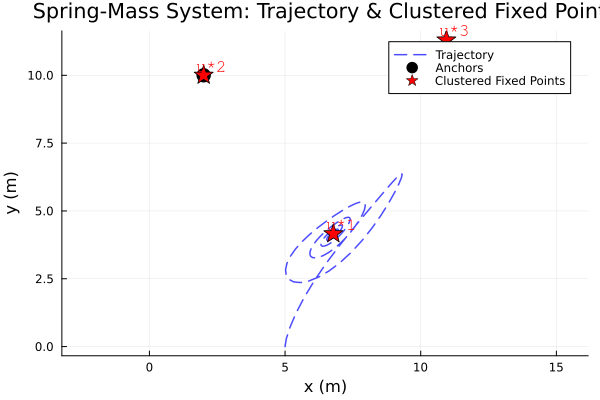
\includegraphics[width=0.75\textwidth]{Problems/Problem13/figures/fixed_points_analysis.png}
    \caption{Simulated mass trajectory and clustered candidate fixed points from the Julia run.}
    \label{fig:p13_fixed_points_analysis}
\end{figure}
